\documentclass{article}
\usepackage[T1]{fontenc}
\usepackage{lato}
\usepackage{graphicx}
\usepackage[unicode=true]{hyperref}
\RequirePackage{polski}
\graphicspath{ {./images/tutorial} }

\title{Laboratorium przetwarzanie obrazów}
\date{}
\author{Radosław Piotrowicz}


\begin{document}
\maketitle

\begin{center}
    \large{ Jak rozszerzyć program o nowe algorytmy }
\end{center}

\newpage
\tableofcontents
\newpage


\section{Gdzie znajdują się interesujące nas rzeczy.}
Jeżeli chcemy dodać nowy algorytm, należy utworzyć 2 nowe pliki oraz zmodyfikować 2 istniejące:
\begin{itemize}
    \item \textbf{Algorithms.hpp} \- dodanie dyrektywy \#include z plikiem nagłówkowym nowego algorytmu
    \item \textbf{App.cpp} \- dodanie do tablicy (vectora) dostępnych algorytmów nowego algorytmu (W metodzie Init okolice linijki 30).
    \item \textbf{<nazwa algorytmu>.hpp} \- stworzenie nowej klasy dziedziczącej po Algorithm oraz nadpisanie metod.
    \item \textbf{<nazwa algorytmu>.cpp} \- implementacja metod.
\end{itemize}

\section{Algorithms.hpp}


\begin{figure}[htbp!]
    \centering
    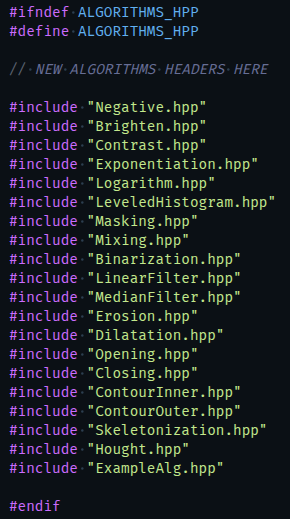
\includegraphics[width=0.8\textwidth]{Algorithms.png}
    \caption{Plik nagłówkowy z algorytmami}
\end{figure}

\newpage

\section{App.cpp}

\begin{figure}[htbp!]
    \centering
    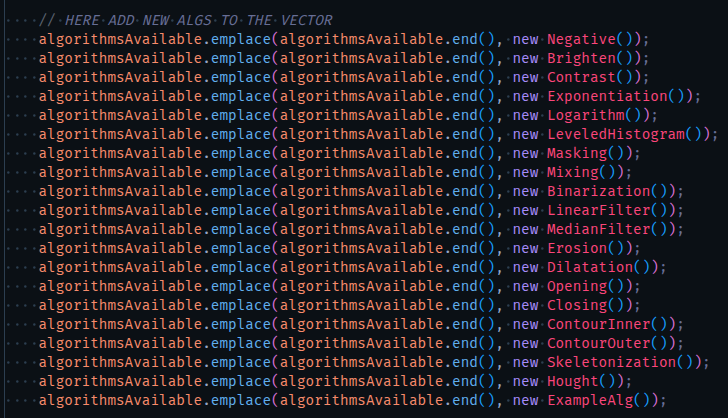
\includegraphics[width=0.8\textwidth]{AlgorithmsVector.png}
    \caption{Sekcja dodawania algorytmów do tablicy}
\end{figure}

Kolejność jest od góry do dołu.


\begin{figure}[htbp!]
    \centering
    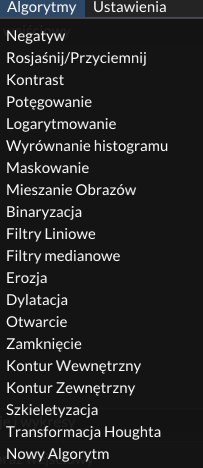
\includegraphics[width=0.8\textwidth]{AlgMenu.png}
    \caption{Menu wyboru algorytmów}
\end{figure}

\newpage

\section{<nazwa algorytmu>.hpp}
Należy utworzyć nowy plik w katalogu \textbf{./include/algorithms}. Przykładowy nowy algorytm jest przedstawiony na rysunku \ref{header}.
Metody od zapisu i wczytania są \textbf{opcjonalne!}.

\newpage

\begin{figure}[htbp!]
    \centering
    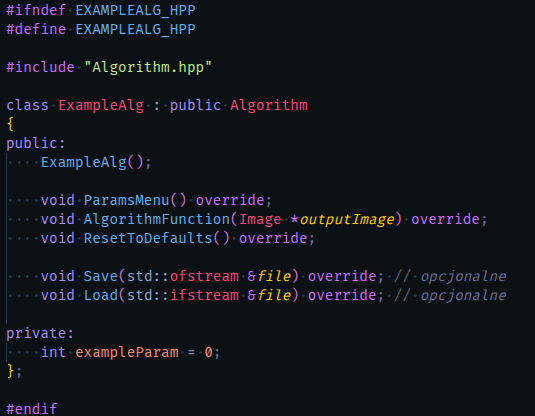
\includegraphics[width=0.8\textwidth]{Header.png}
    \caption{Przykładowy plik nagłówkowy nowego algorytmu}
    \label{header}
\end{figure}

Można też utworzyć klasę pośrednią, jeżeli kilka algorytmów będzie miało takie same parametry.
Przykładem jest \textbf{MorphologicAlgorithm.hpp}.

\section{<nazwa algorytmu>.cpp}
Tutaj jest najwięcej do zrobienia.

\subsection{Wersja minimum}
Na rysunku \ref{minimum} przedstawiono minimum co trzeba zrobić, aby algorytm zadziałał.

\begin{figure}[htbp!]
    \centering
    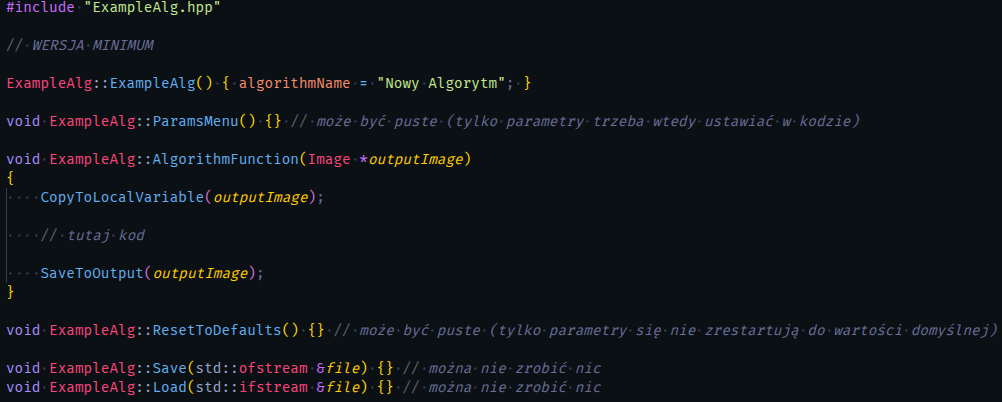
\includegraphics[width=0.8\textwidth]{Minimum.png}
    \caption{Minimalna implementacja}
    \label{minimum}
\end{figure}

\subsection{Wersja pełna}
Na rysunku \ref{full} przedstawiono przykładową implementację wszystkich metod.

\begin{figure}[htbp!]
    \centering
    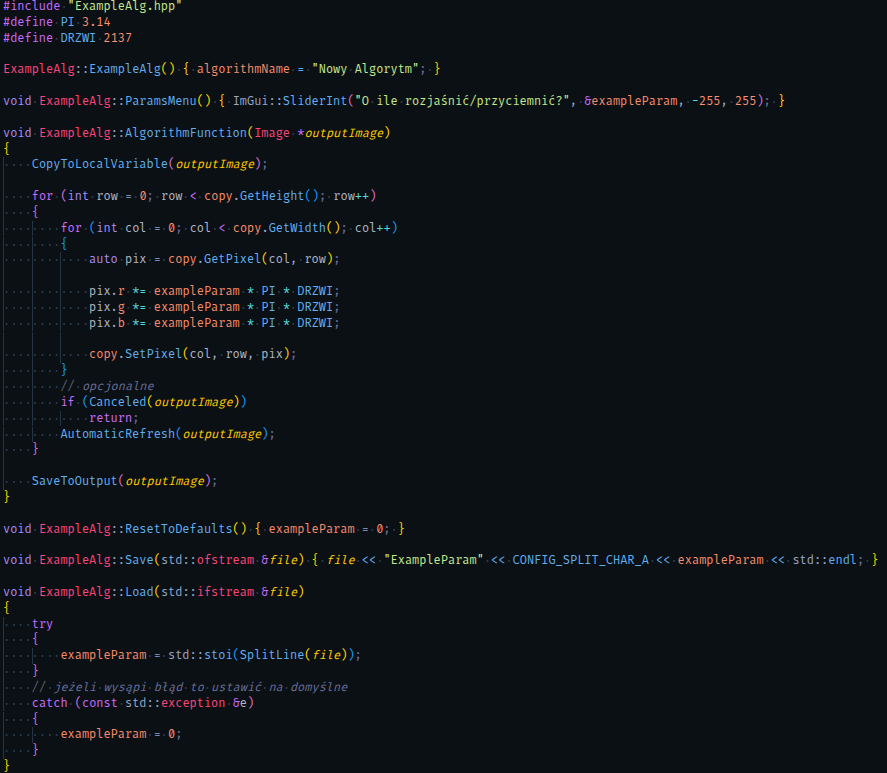
\includegraphics[width=0.8\textwidth]{Full.png}
    \caption{Pełna implementacja}
    \label{full}
\end{figure}

\textbf{Ważne}
\begin{itemize}
    \item Automatyczne odświeżanie oraz Anulowanie są opcjonalne.
    \item Można posiłkować się metodami od parametrów, resetu, zapisu i odczytu z innych algorytmów jako przykładów (powinno tam być sporo przypadków).  
\end{itemize}

\subsection{Parametry}
Tutaj jest dodatkowy opis oraz kilka przykładów graficznego menu do ustawienia parametrów. Bazowo (jeżeli zostawimy metodę od parametrów pustą) okienko będzie wyglądać jak na rysunku \ref{noparams}.
\newpage

\begin{figure}[htbp!]
    \centering
    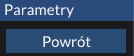
\includegraphics[width=0.8\textwidth]{NoParams.png}
    \caption{Puste}
    \label{noparams}
\end{figure}

Jeżeli jednak chcemy dorobić menu graficzne poniżej jest przedstawione kilka przykładów:
\subsubsection{Pojedynczy parametr.}
Dla niektórych algorytmów wystarcza obsługa tylko jednego parametru na przykład:
\newline
\textbf{ImGui::SliderInt("O ile rozjaśnić/przyciemnić?", \&params.value, -255, 255)}
\newline
Najpierw jest opis slidera, potem wartość, do której zapisany będzie wynik, następnie ograniczenia dolne i górne.
\newline
A tak będzie wyglądało okienko.
\begin{figure}[htbp!]
    \centering
    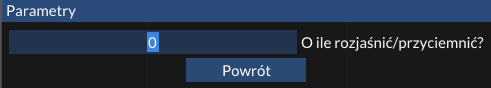
\includegraphics[width=0.8\textwidth]{SimpleParam.png}
    \caption{Pojedynczy parametr}
\end{figure}

\subsubsection{Kilka parametrów}
Czasami może być potrzebne kilka parametrów do algorytmu. Takich jak rodzaj metody lub liczba progów.
Wtedy można do zrobić w ten sposób.

\newpage

\begin{figure}[htbp!]
    \centering
    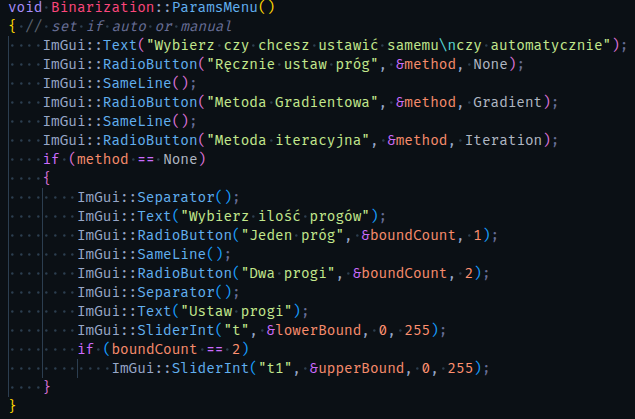
\includegraphics[width=0.8\textwidth]{Binarization.png}
    \caption{Kilka parametrów}
\end{figure}

Na początku metody pomocniczej znajduje się pierwszy wybór (metody), obsługiwany jest przez funkcje \textbf{ImGui::RadioButton()}.
Funkcja ta przyjmuje jako parametry:
\begin{itemize}
    \item  \textbf{const char *label} \- nazwa opcji
    \item  \textbf{int *v} \- wskaźnik do zmiennej z obecnie wybranym stanem
    \item  \textbf{int v\_button} \- numer stanu przypisany do opcji (najlepiej zdefiniowany w enum)
\end{itemize}

\textbf{ImGui::SameLine()} \- informuje, żeby umieścić elementy w tej samej linii.
\newline
\textbf{ImGui::Separator()} \- tworzy linię separującą elementy.
\newline
Następnie znajduje się kolejny wybór (ilości progów), zrobiony analogicznie do wyboru metody. Jedak pojawi się on tylko wtedy gdy ustawiamy progi ręcznie.
Również, jeżeli ustawiamy progi ręcznie pojawią się dwa slidery do wyboru wartości progu.
\newpage
Okienko będzie wyglądało tak:

\begin{figure}[htbp!]
    \centering
    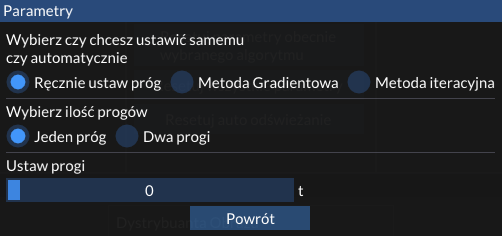
\includegraphics[width=0.8\textwidth]{BinarizationP.png}
    \caption{Okienko kilku parametrów}
\end{figure}

\subsubsection{Parametry tabelkowe}
Przy niektórych algorytmach parametrem jest macierz (maska albo element strukturalny).

\begin{figure}[htbp!]
    \centering
    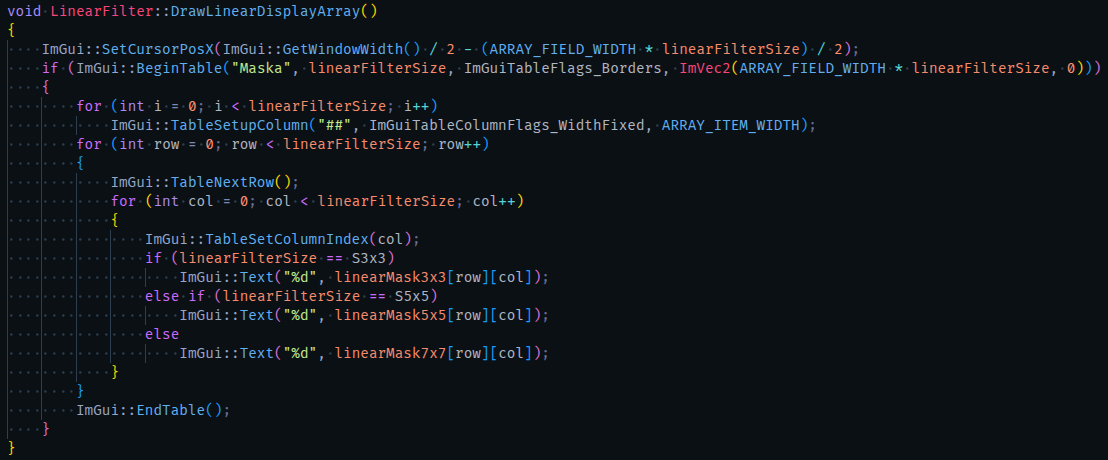
\includegraphics[width=0.8\textwidth]{InputArrayExample.png}
    \caption{Tabelka w kodzie}
\end{figure}

Aby rozpocząć tabelkę, należy użyć funkcji ImGui::BeginTable(), i musi się ona znajdować w instrukcji warunkowej.
Funkcja ta przyjmuje następujące parametry:
\begin{itemize}
    \item \textbf{const char *str\_id} \- nazwa tablicy
    \item \textbf{int columns} \- ilość kolumn
    \item \textbf{ImGuiTableFlags flags} \- flagi dotyczące wyglądu tablicy
    \item \textbf{const ImVec2 \&outer\_size} \- rozmiar tablicy
    \item \textbf{float inner\_width} \- wewnętrzna szerokość komórek
\end{itemize}
W naszym przypadku interesować będą nas pierwsze 3-4 parametry.

Następnie należy w pętli podwójnej utworzyć wszystkie elementy.

W zewnętrznej pętli (dla wierszy) używamy ImGui::TableNextRow() aby przejść do kolejnego wiersza.
Następnie w wewnętrznej pętli (dla kolumn) ustawiamy kursor na kolumnę przy użyciu ImGui::TableSetColumnIndex(col) i dodajemy element.
\newline
Aby dodać nowy element, można użyć różnych elementów na przykład:
\begin{itemize}
    \item ImGui::Text() - do wyświetlenia elementu bez możliwości wprowadzenia.
    \item ImGui::InputInt() - do wprowadzenia liczby całkowitej z powiązaniem do elementu o odpowiednim indeksie.
    \item ImGui::Checkbox() - do oznaczenia elementu, którego wartości mogą przyjąć true/false.
\end{itemize}

Tak będą wyglądać tablice w kolejności takiej, jak na liście:

\newpage

\begin{figure}[htbp!]
    \centering
    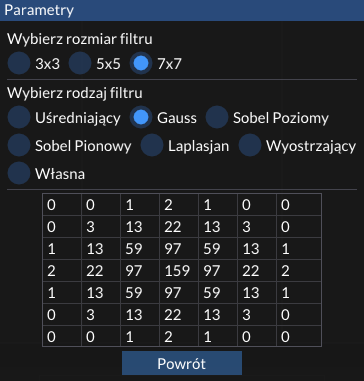
\includegraphics[width=0.8\textwidth]{FilterP.png}
    \caption{Tablica z samym wyświetlaniem zawartości}
\end{figure}

\begin{figure}[htbp!]
    \centering
    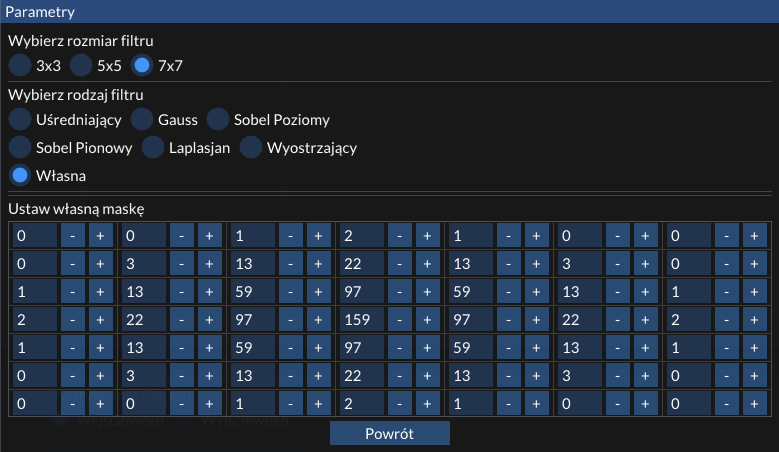
\includegraphics[width=0.8\textwidth]{FilterPC.png}
    \caption{Tablica z wprowadzaniem liczb całkowitych}
\end{figure}

\newpage

\begin{figure}[htbp!]
    \centering
    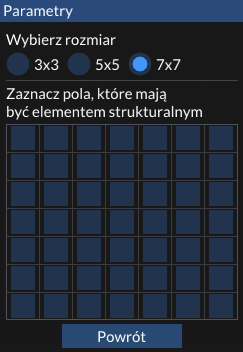
\includegraphics[width=0.8\textwidth]{Element.png}
    \caption{Tablica z checkboxami}
\end{figure}

Na koniec tablice należy zakończyć używając ImGui::EndTable().

\textbf{Dodatkowe uwagi:}
\begin{itemize}
    \item Jeżeli tablica ma służyć do wprowadzania danych należy użyć \textbf{ImGui::PushID(nr wiersza)} - przed ImGui::TableNextRow() i \textbf{ImGui::PopID()} - po wewnętrznej pętli.
    \item Jeżeli ustawiamy ID należy najpierw użyć \textbf{std::string s = "\#\#" + std::to\_string(col)}, aby ustalić to ID, a następnie przekazać je do funkcji od elementu na przykład \textbf{ImGui::Checkbox(s.c\_str(), \&a3x3[row][col])}.
    \item Jeżeli nie potrzebujemy opisów kolumn, można użyć \textbf{ ImGui::TableSetupColumn("\#\#")} dla każdej kolumny.
    \item Jeżeli chcemy ustawić szerokość elementu użyjemy \textbf{ImGui::TableSetupColumn("\#\#", ImGuiTableColumnFlags\_WidthFixed, ARRAY\_ITEM\_WIDTH)} \textbf{Tablica powinna mieć podany stały rozmiar w ImGui::BeginTable()}.
    \item Jeżeli tablica nie ma ustawionego rozmiaru na początku można określić szerokość elementu możemy użyć \textbf{ImGui::PushItemWidth(ARRAY\_INPUT\_WIDTH)}.
    \item Przykłady metod obsługujących tabelki można znaleźć w plikach \textbf{LinearFilter.cpp}, \textbf{MedianFiler.cpp}, \textbf{MorphologicAlgorithm.cpp}.
\end{itemize}

\section{ImGui}
W tej sekcji opisze przydatne informacje dotyczące użytej biblioteki graficznej.
\subsection{ImGuiDemo}
Do programu dołączone jest ImGuiDemo, które zawiera przykłady możliwości biblioteki graficznej.
\newline
Znajduje się ono w sekcji \textbf{Pomoc->Pokaż ImGuiDemo}
\newline
Okno wygląda tak:
\begin{figure}[htbp!]
    \centering
    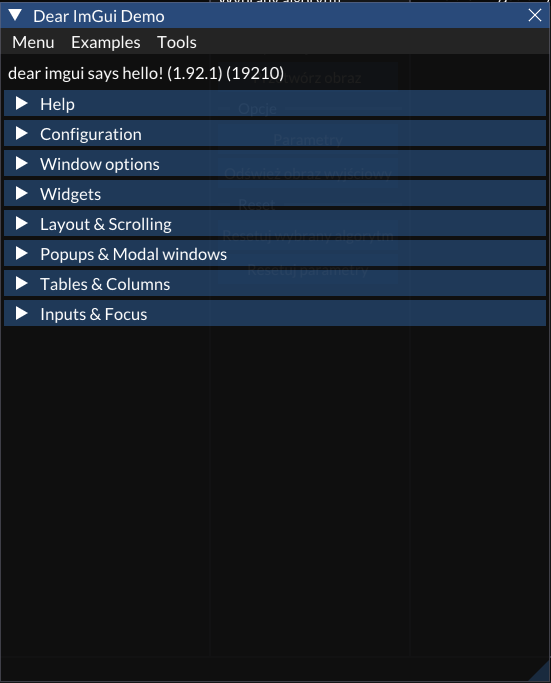
\includegraphics[width=0.8\textwidth]{ImGuiDemo.png}
    \caption{Okno ImGuiDemo}
\end{figure}

\newpage

Przykłady w kodzie znajdują się w pliku \textbf{imgui\_demo.cpp.} Plik ten znajduje się w folderze ImGui.
\newline
W tym pliku powinno znajdować się wszystko, co może być potrzebne przy zapoznawaniu się z biblioteką. Ponadto twórcy ImGui zachęcają do zachowania tego pliku w projektach w celu posiadania przykładów implementacji funkcjonalności.

\begin{figure}[htbp!]
    \centering
    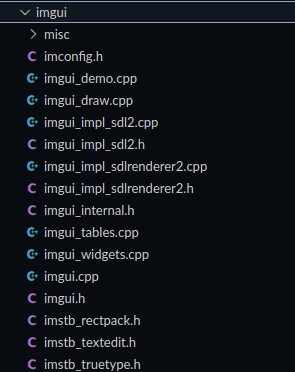
\includegraphics[width=0.8\textwidth]{ImGuiDir.png}
    \caption{Folder ImGui}
\end{figure}

\subsection{Link do biblioteki}
Na końcu zostawiam link do Githuba, z biblioteką. Znajdują się tam wszystkie potrzebne informacje.
\newline
\textbf{Github:} \href{https://github.com/ocornut/imgui}{https://github.com/ocornut/imgui}

\end{document}
